%%____________________________________________________________________________||
\section{Aggregate signal regions}
\label{sec:aggregate-signal-regions}

Inclusive searches for new physics typically use fine categorisation to allow
sensitivity to a wide range of models. However, this can make the use
of the search for re-interpretation impractical. 
This section describes how this categorisation may be simplified without breaking the correlation 
between the bins by defining aggregate regions which are disjoint, 
contiguous and cover the full signal region.

Considering the simplified likelihood defined in Equation~\ref{eq:full-likelihood},
the likelihood for aggregate regions may be written by replacing the 
background predictions as shown in Equation~\ref{eq:b-agg},

\begin{align}
b_{i} + \theta_i \rightarrow b_I + \theta_I \equiv \sum_{i}^{N_i}(b_{i}) + \theta_I
\label{eq:b-agg}
\end{align}

where the sum is over all regions being aggregated into regions $I$.
Note that all nominal regions must be included in the aggregate likelihood.
Similarly, the signal counts, observations and covariance used in Equation~\ref{eq:full-likelihood} are
replaced with those from the aggregate regions. These may be derived, approximately, using the predictions and covariance
of the nominal signal regions (discussed in Section~\ref{sec:simplified-likelihood}).
Equation~\ref{eq:agg-cov} shows how the predictions and covariance in the aggregate
regions are related to those of the nominal region. The approximation in using Equation~\ref{eq:agg-cov} to 
define the aggregate region relies on the same conditions 
on the nuisances outlined in Section~\ref{sec:simplified-likelihood}. 

\begin{align}
b_{I} = \sum_i b_{i} && V_{IJ}=\sum_{ij}V_{ij}
\label{eq:agg-cov}
\end{align}

where the sums are over all regions being aggregated into regions $I,J$. 

\subsection{Example of the use of aggregate regions}
\label{sec:agg-toy}

The same toy model is considered as in Section~\ref{sec:sl-toy}. From Figure~\ref{fig:toy-example}
it is clear that only search regions 7 and 8 exhibit large contributions from the signal
model. One may therefore expect that regions 1-6 can be neglected when setting limits. 
However, as these bins are correlated, if regions 1-6 are not considered information 
on the nuisances in the regions with large signal contributions is lost. 
Alternatively, the regions 1-6 may be aggregated using the covariance matrix shown in 
Figure~\ref{fig:covariance} using Equation~\ref{eq:agg-cov}. The resulting covariance
between the aggregate regions is shown in Figure~\ref{fig:agg-covariance}.

\begin{figure}[hbt]
  \begin{center} 
   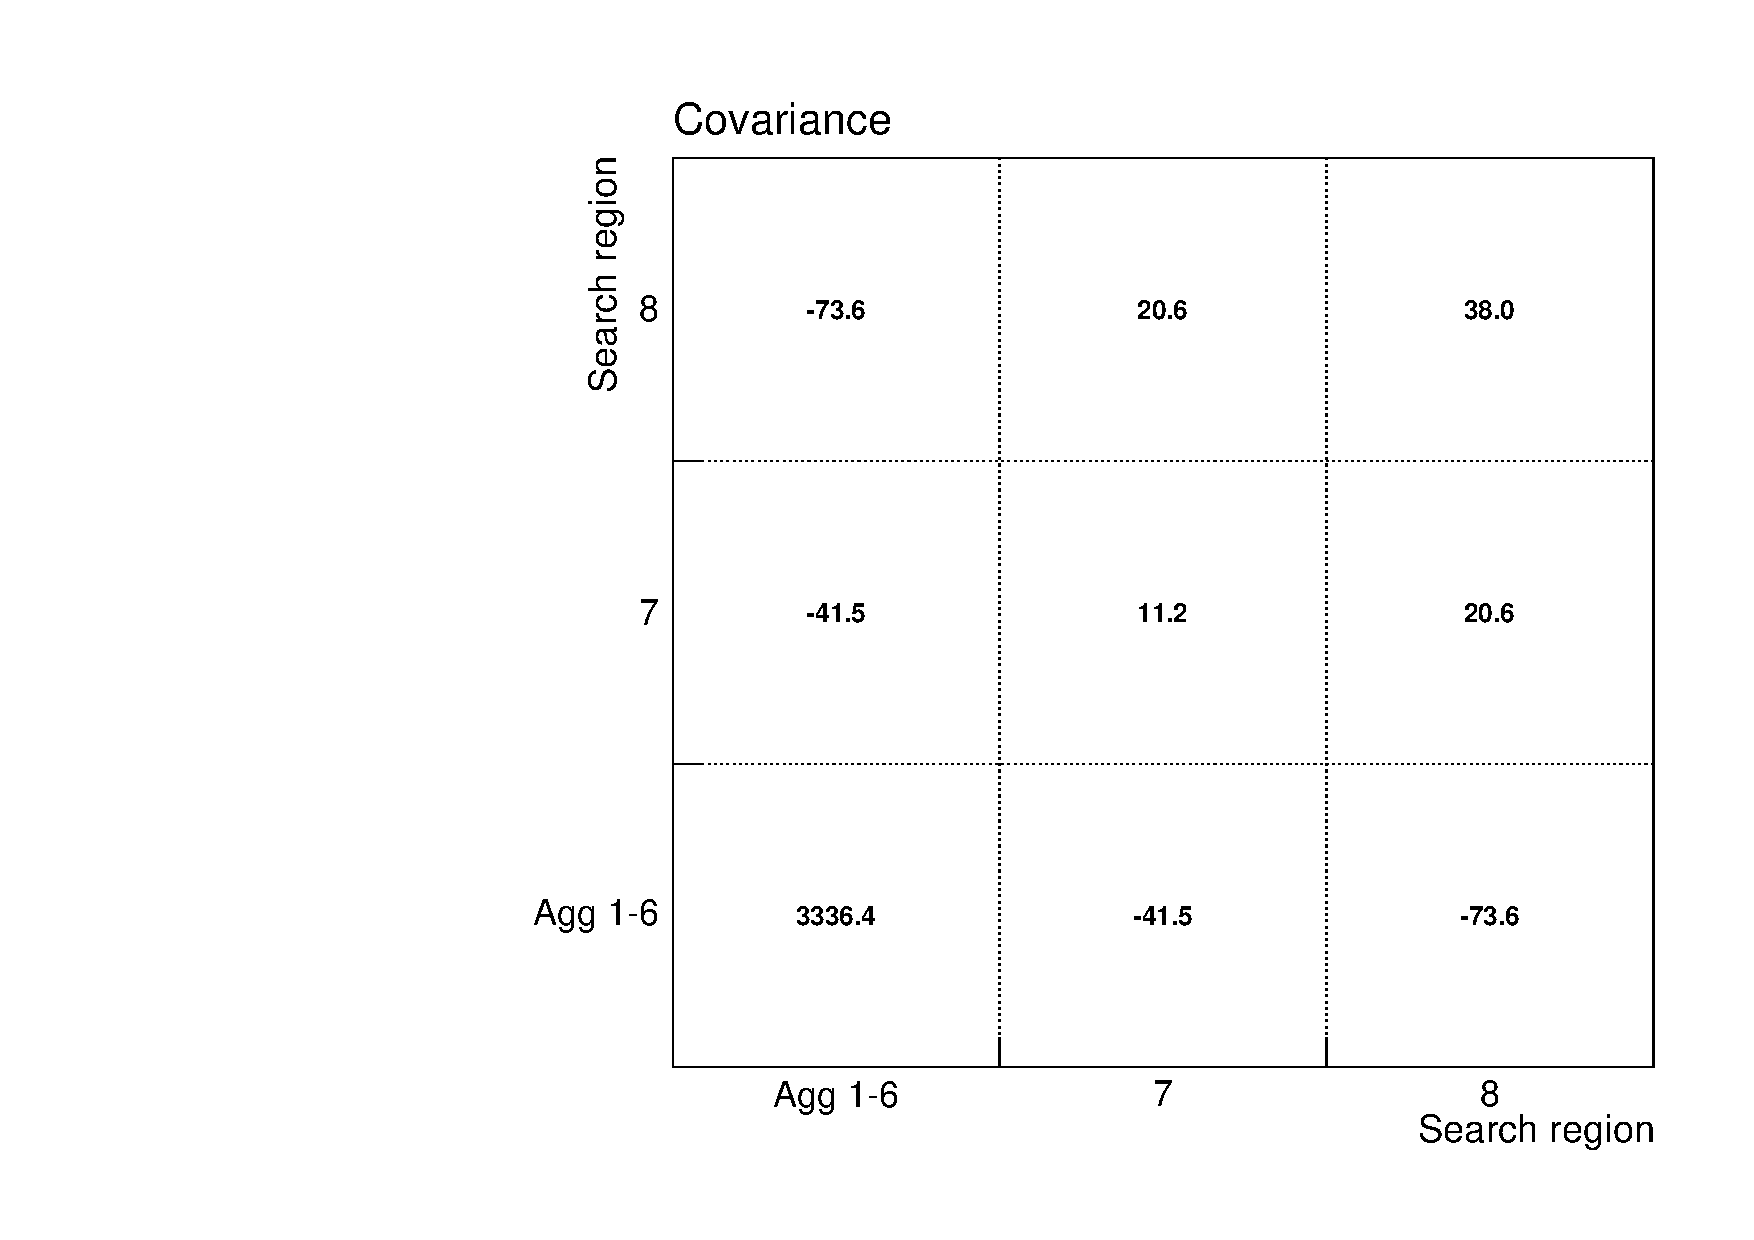
\includegraphics[width=1.5\cmsFigWidth]{figures/agg_htsearch_covariance.pdf}
   \caption{Covariance between the total rate of background contributions expected in each of the aggregated search regions}
   \label{fig:agg-covariance} 
  \end{center}
\end{figure}

Figure~\ref{fig:agg-likelihoodscan} shows the value of $q(\mu)$ as a function of $\mu$. The values when $q(\mu)$ 
is defined using the likelihood of Equation~\ref{eq:full-likelihood} for the nominal signal region, the aggregated signal
regions described above, and considering search regions 7 and 8 only are shown. The aggregated regions show
good agreement compared to the nominal while neglecting the regions 1-6 is shown to introduce a considerable
bias in the estimate of $\hat{\mu}$. In addition, the width of the likelihood curve when neglecting these regions is considerably
larger, implying a larger uncertainty estimate on $\mu$. This can be expected from the loss of information on
the systematic uncertainties when search regions 1-6 are neglected. In this case the limit will be considerably
weaker than if all regions are considered. Generically, the impact of removing regions
will be dependant on the size of the systematic uncertainties and correlations between the regions used and those
dropped.

\begin{figure}[hbt]
  \begin{center} 
   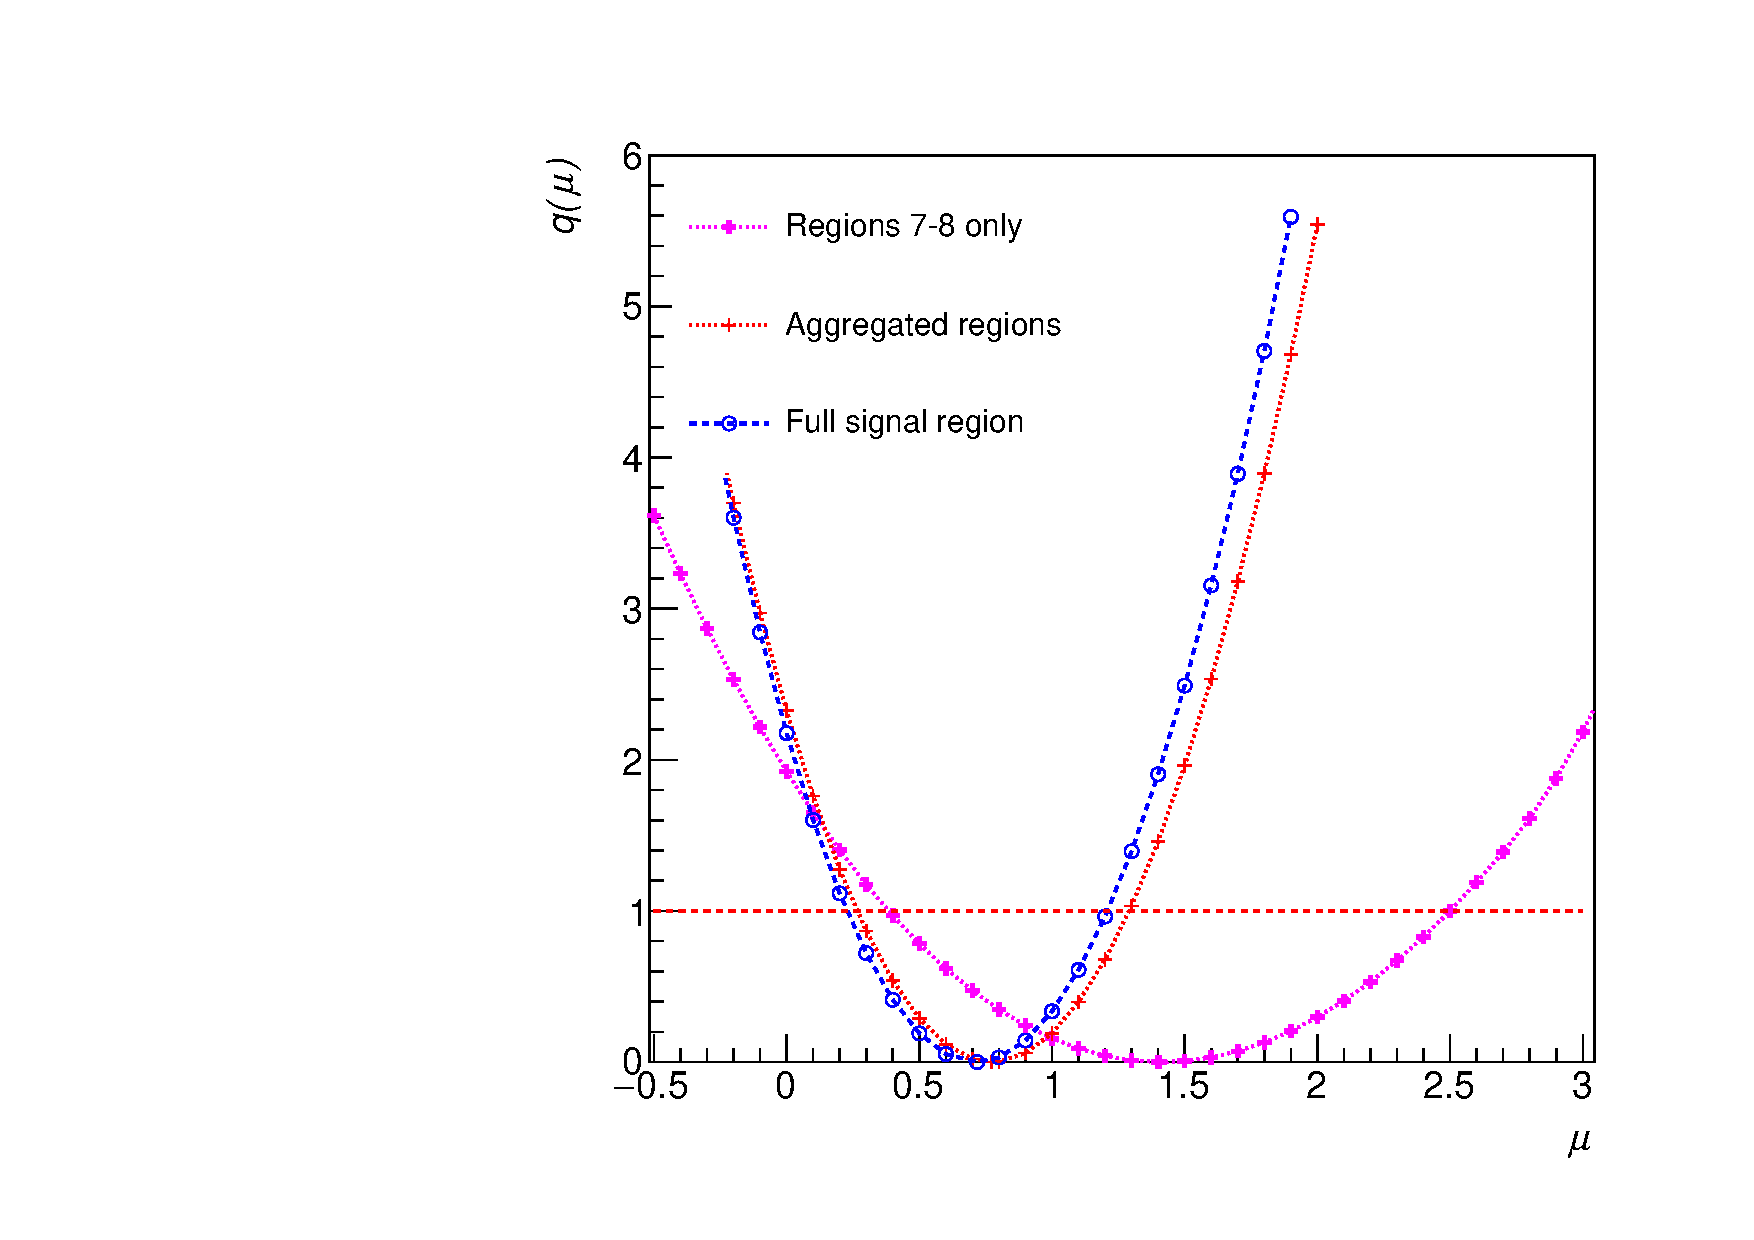
\includegraphics[width=1.5\cmsFigWidth]{figures/r_agg.pdf}
   \caption{The value of $q(\mu)$ defined using the simplified likelihood using the full signal region (open blue points), the aggregated signal region (thin red crosses),
   and regions 7-8 only (open magenta crosses).}
   \label{fig:agg-likelihoodscan} 
  \end{center}
\end{figure}
